\documentclass{article}

\usepackage[french]{babel}
\usepackage[utf8]{inputenc}
\usepackage[T1]{fontenc}
\usepackage{verbatim}
\usepackage{amsmath}
\usepackage{geometry}

\usepackage[final]{pdfpages}

%% Si ca ne compile pas chez vous, mettez la ligne suivante en commentaire
%\usepackage{tikz}

%\date{}
\author{Groupe :\\ \\Benbrahim Douha\\Meunier Bastien\\Wang Miao }
\title{Compte rendu SGBD \\ Gestion d'un club sportif}


\begin{document}
\maketitle
\newpage
\section{Introduction}

Afin de garder les information sur ses membres et sur son foncionnement, un club sportif peut être amener à utiliser une base de données. Le sujet que nous avons choisi consite en l'implémentation d'une base de données pour un club de basket ball.
Tout d'abord nous avons dû créer un modèle conceptuel puis relationnel afin de représenter le club sportif. Puis, après nous être assurer d'avoir un modèle en 3eme forme normale nous avons commencé l'implémentation. 
Ainsi, nous avons dû créer deux fichiers afin de créer la base : base.sql et données.sql qui nous ont ensuite servi à tester nos requêtes.
Puis, nous avons créer les requêtes et enfin l'interface graphique permettant leur utilisation. Pour celle-ci nous avons choisi jdbc car nous avons une bonne maîtrise du java.


\section{Modèle conceptuel}

Pour la modélisation EA nous avons créer 7 entités ainsi que 7 relations. Dans un premier temps nous avions créer une relation rencontre. Mais finalement nous avons opté pour une entité ... %Je ne sais plus. Mis à part le fait que le prof a demandé, pourquoi on a fait une entité finalement?
Nous avons cependant laissé "Cumul_Points_Marqués" ainsi que "Cumul_Fautes" dans la relation entre joueur et match. En effet, ces deux caractéristiques dépendent de ces 2 entités.


 
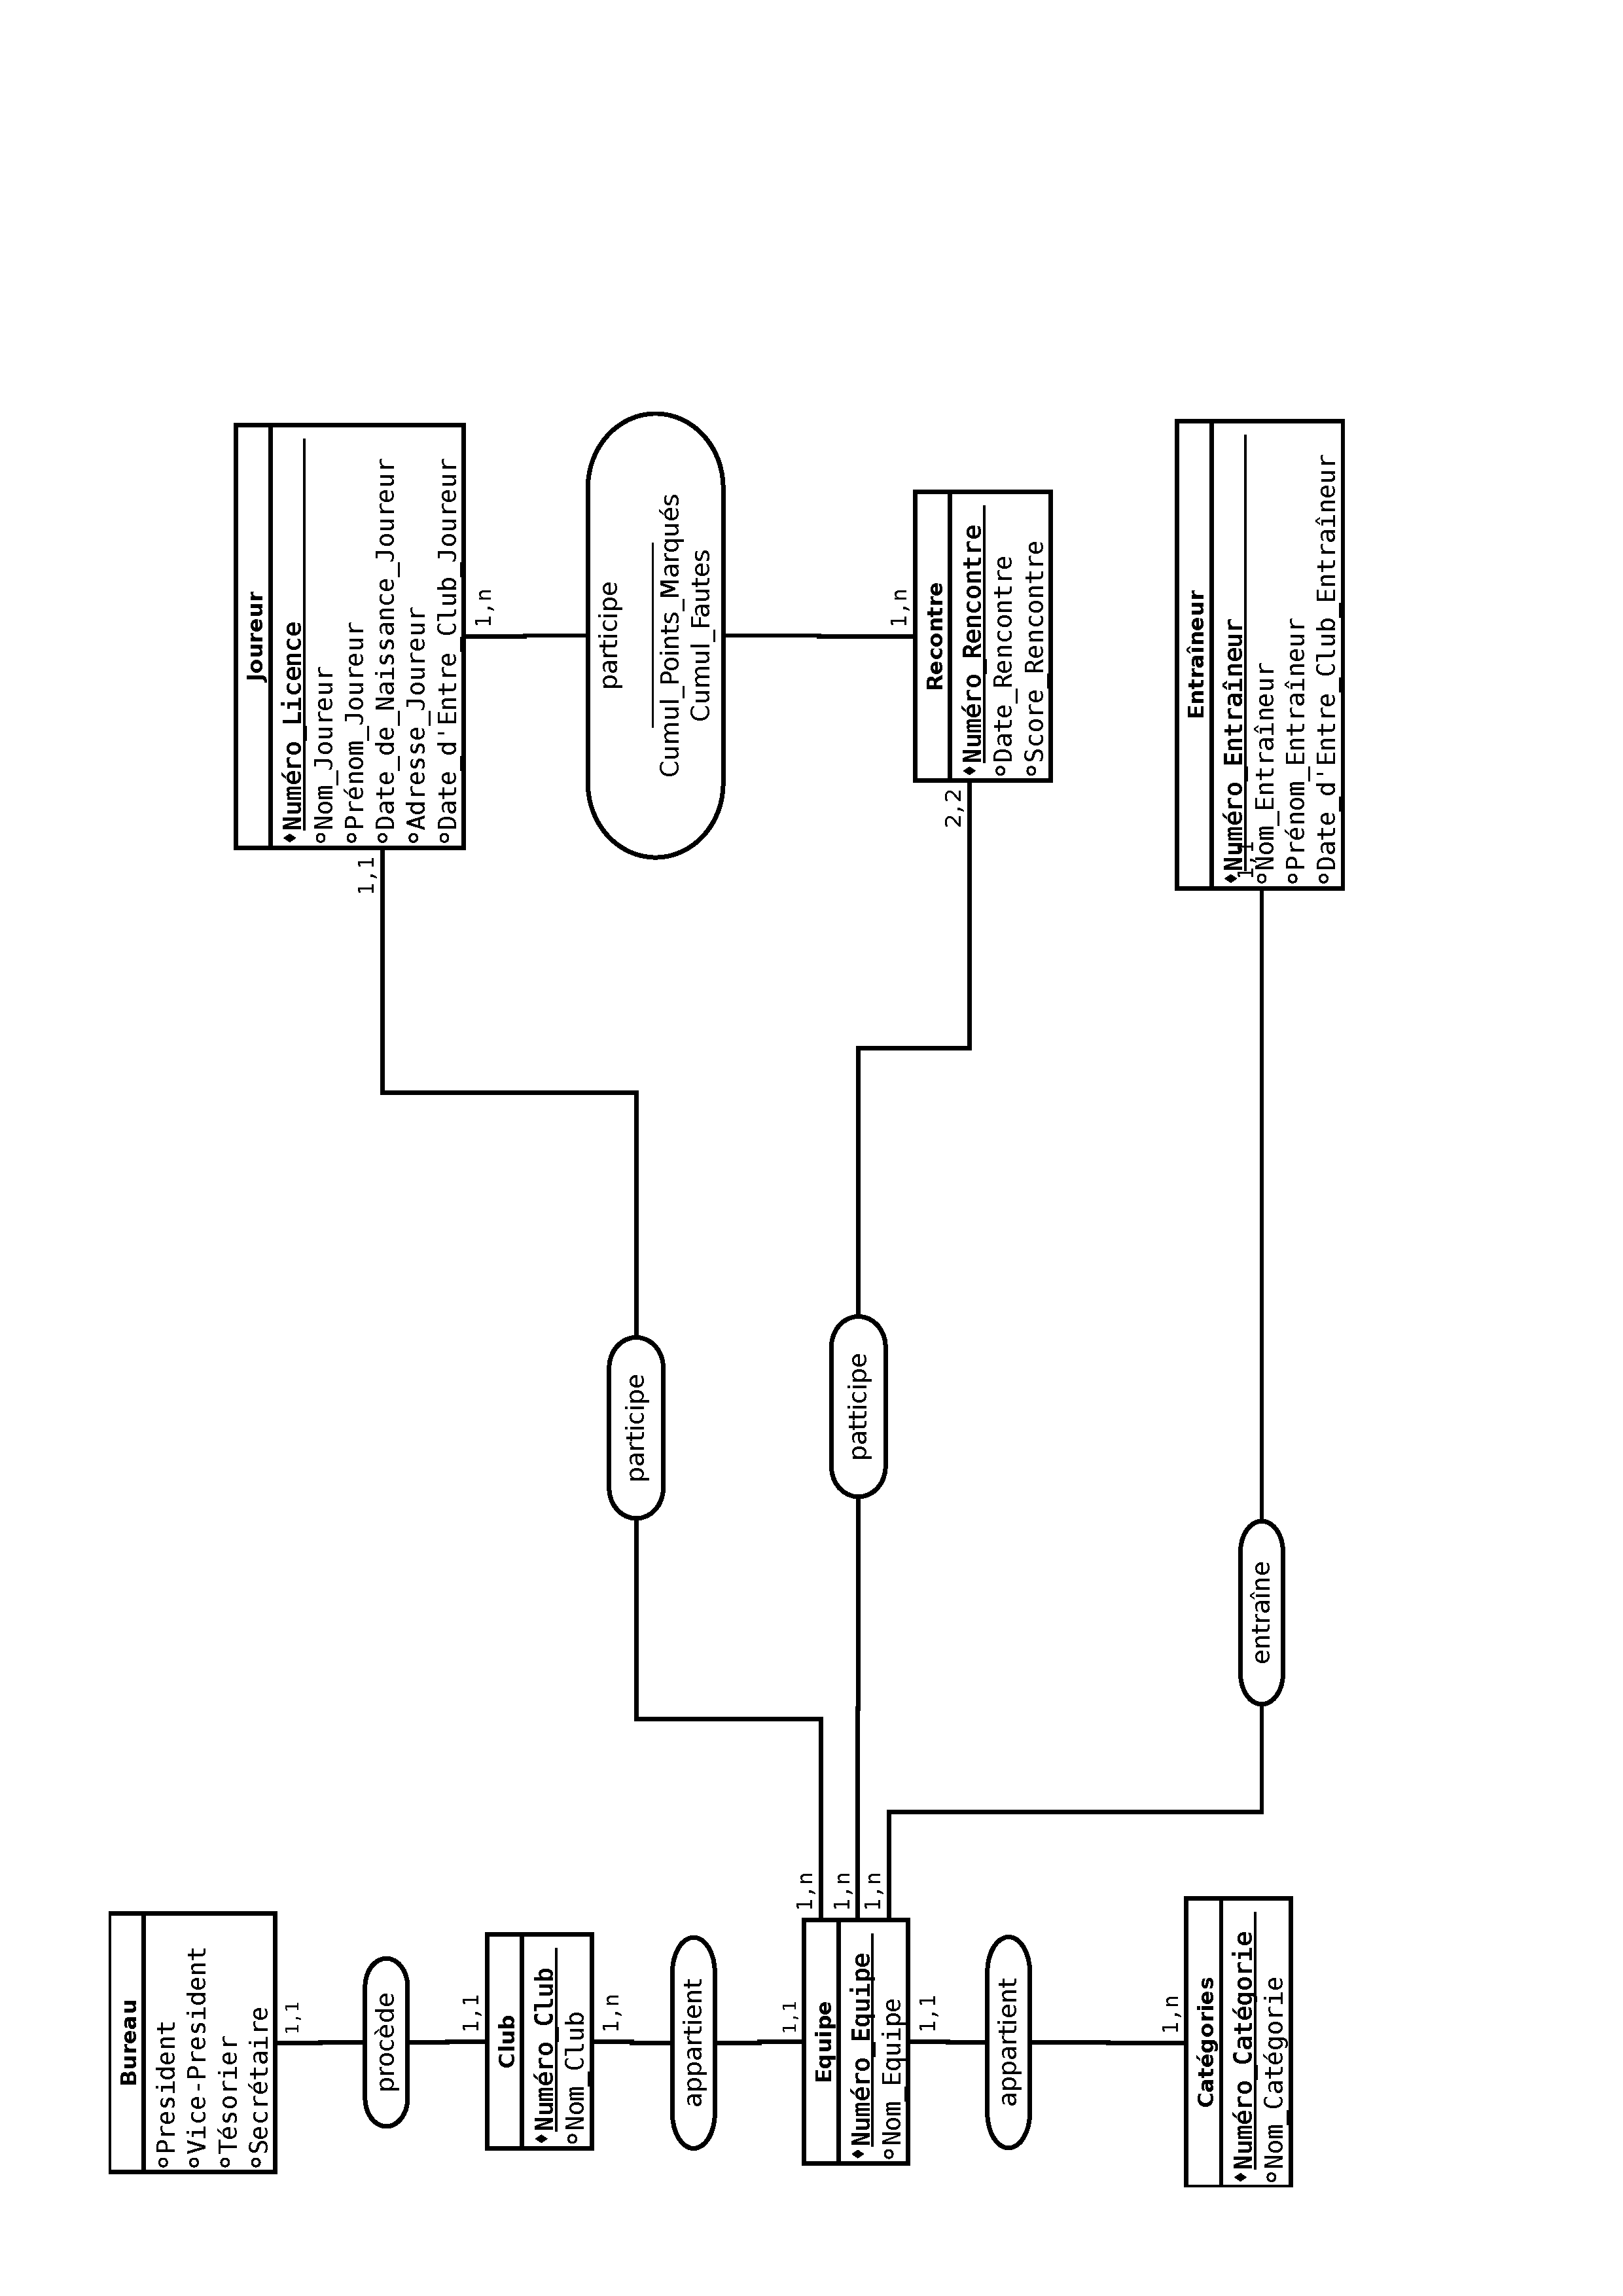
\includepdf[page=1]{Basketball_EA.pdf}

\section{Modèle relationnel}
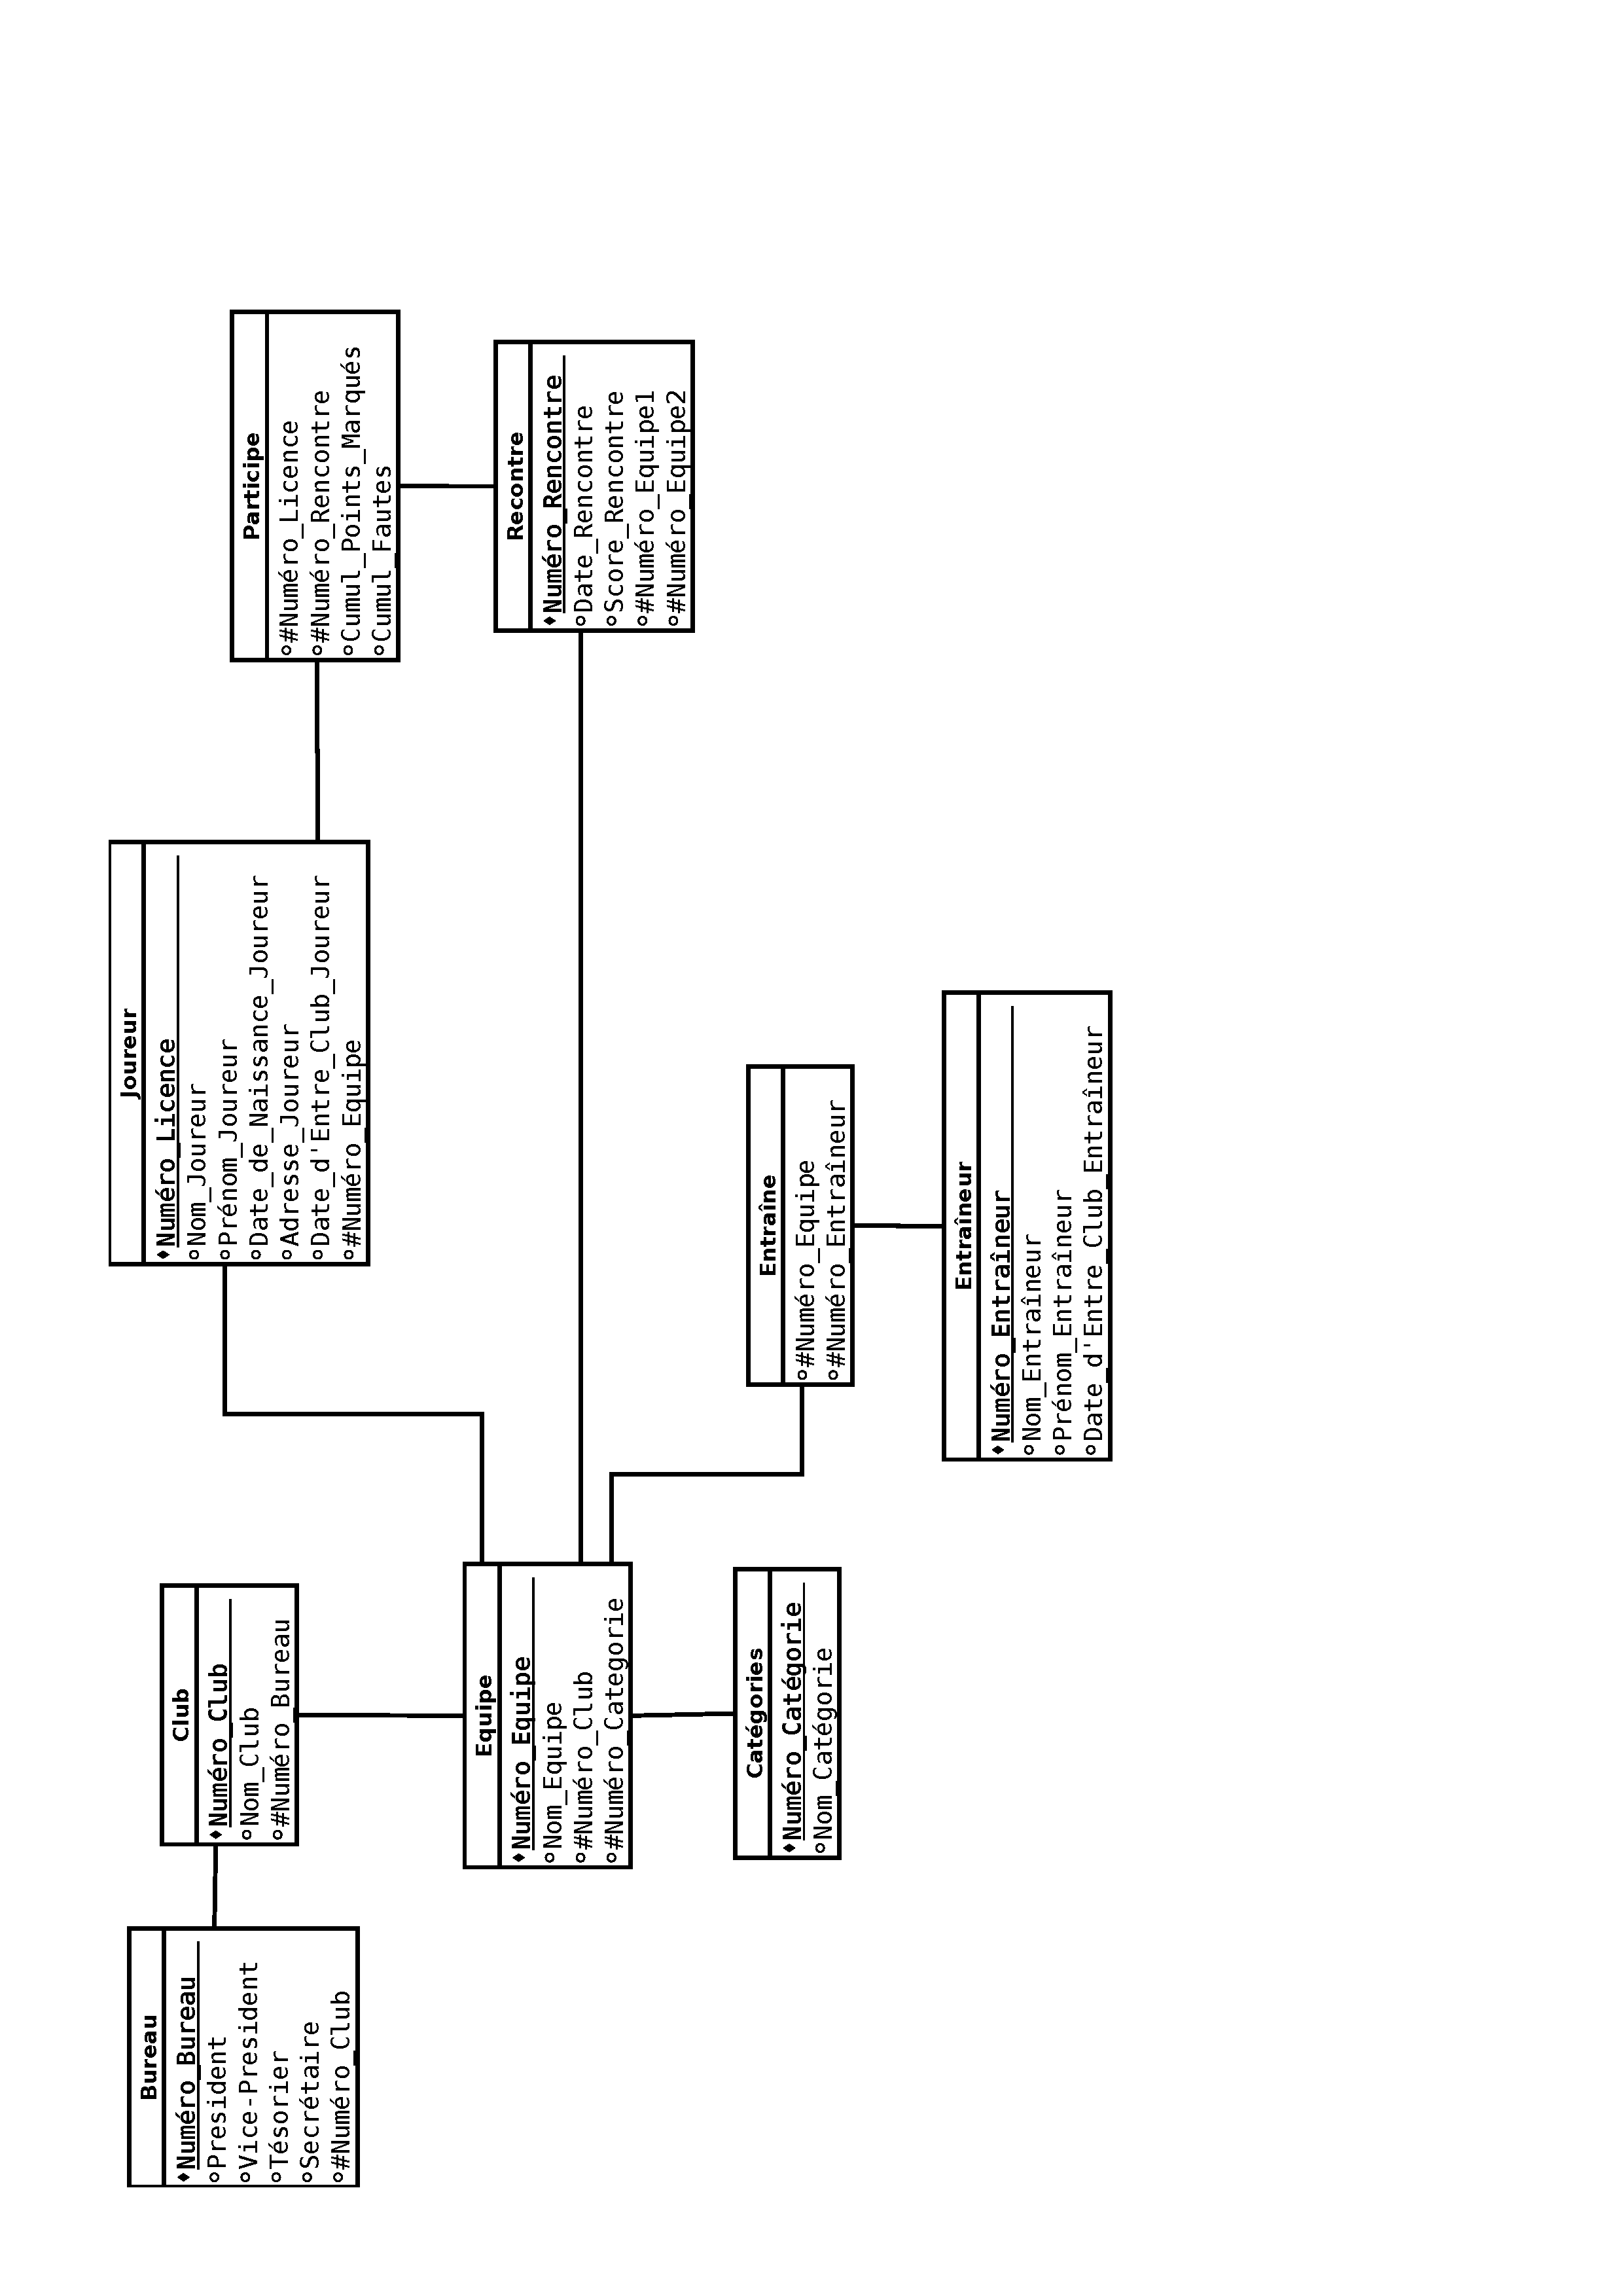
\includepdf[page=1]{Basketball_Relationnel.pdf}




\subsection*{}


\section*{}
\subsection*{}


\subsection*{}

\end{document}
